%%
%% $Id$
%%
%% Copyright (c) 2007-2008 Christian Fehler
%% Copyright (c) 2007-2008 Benjamin Mies
%%


\chapter{Grammatiken}\label{Grammars}

Eines der Hauptthemen, mit denen sich das Fach Grundlagen der Informatik
beschäftigt, sind Grammatiken. Daher ist dieses Themengebiet auch Bestandteil
unseres Lernwerkzeugs geworden. Der Benutzer muss die Möglichkeit haben, eine
Menge von Terminalzeichen und Nichtterminalzeichen anzugeben, ebenso wie ein
Startsymbol festzulegen. Dies haben wir durch Eingabefelder realisiert, hinter
welchen entsprechende Parser liegen. Die Parser werden detailiert im Kapitel
\ref{Parser} erläutert.\vspace{10pt}

\begin{figure}[h!]
\begin{center}
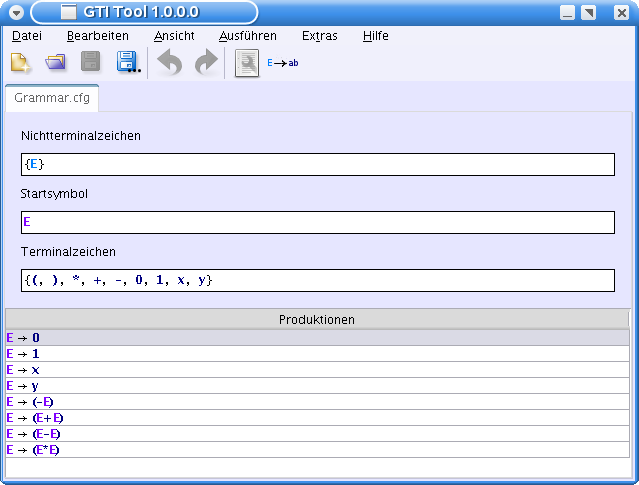
\includegraphics[width=12cm]{../images/cfg_example.png}
\caption{Grammatik}
\label{FigureProduction}
\end{center}
\end{figure}
\vspace{10pt}

Zur Darstellung der Produktionen wird eine Listenansicht verwendet, wobei die
Produktionen als PrettyString angezeigt werden. Das bedeutet, dass man die
verschiedenen Symbole (Terminalzeichen, Nichtterminalzeichen, Startsymbol) in den
Farben dargestellt bekommt, die man in den Einstellungen dafür vergeben hat. Wir
hoffen, dadurch eine bessere Übersichtlichkeit in den einzelnen Produktionen für
den Benutzer geschaffen zu haben (siehe Abbildung
\ref{FigureProduction}).\vspace{10pt}

Als Hilfestellung beim Anlegen von neuen Produktionen wird die aktuelle
Konfiguration der Grammatik oberhalb der existierenden Produktionen
angezeigt.\vspace{10pt}


\begin{figure}[h!]
\begin{center}
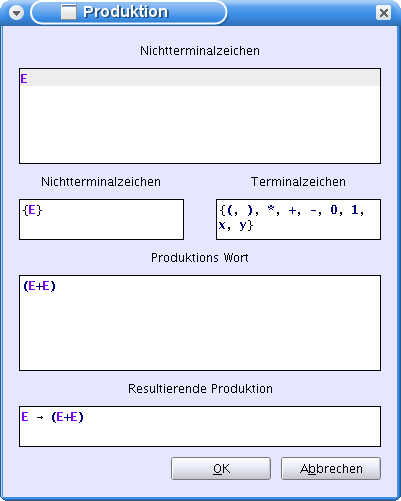
\includegraphics[width=8cm]{../images/production_dialog.png}
\caption{Grammatik - Produktion anlegen}
\label{FigureAddProduction}
\end{center}
\end{figure}
\vspace{10pt}

Wir haben versucht, das Anlegen einer neuen Produktion so intuitiv wie möglich
zu gestalten. Der Benutzer kann das Nichtterminalzeichen, welches die linke
Seite der Produktion repräsentiert, anhand einer Liste der
verfügbaren Symbole auswählen. Die Eingabe der rechten Seite ist
wieder über ein Textfeld, mit entsprechendem Parser, realisiert
worden. Oberhalb des Eingabefeldes wird dabei angezeigt, welche Symbole zur
Konstruktion des Wortes der Satzform zur Verfügung stehen. Als weitere
Hilfestellung haben wir unterhalb des Eingabefeldes einen Bereich angelegt,
in welchem die resultierende Produktion angezeigt wird. So kann der
Benuzter jederzeit überprüfen, ob das Ergebnis seinen
Vorstellungen entspricht. In Abbildung \ref{FigureAddProduction}
sieht man den Dialog, welcher Verwendet wird um Produktionen
anzulegen und zu bearbeiten.\vspace{10pt}

Der Benutzer hat auch die Möglichkeit, seine definierte Grammatik zu validieren.
Kapitel \ref{Interaction} beschreibt die Umsetzung im Detail.\vspace{10pt}
